\documentclass{beamer}

\setbeamertemplate{navigation symbols}{}
\setbeamertemplate{footline}{\insertpagenumber}
% This file is a solution template for:

% - Giving a talk on some subject.
% - The talk is between 15min and 45min long.
% - Style is ornate.



% Copyright 2004 by Till Tantau <tantau@users.sourceforge.net>.
%
% In principle, this file can be redistributed and/or modified under
% the terms of the GNU Public License, version 2.
%
% However, this file is supposed to be a template to be modified
% for your own needs. For this reason, if you use this file as a
% template and not specifically distribute it as part of a another
% package/program, I grant the extra permission to freely copy and
% modify this file as you see fit and even to delete this copyright
% notice.


\mode<presentation>
{
  %\usetheme{Warsaw}
  %\usetheme{Montpellier}
  \usetheme{Singapore} % Malmoe}
  % or ...

  \setbeamercovered{transparent}
  % or whatever (possibly just delete it)
}

\input{header}
\usepackage[english]{babel}
% or whatever

\usepackage[mathletters]{ucs}
\usepackage[utf8x]{inputenc}

\usepackage{times}
\usepackage[T1]{fontenc}


% Or whatever. Note that the encoding and the font should match. If T1
% does not look nice, try deleting the line with the fontenc.

\usepackage{tikz}
\usepackage{pgflibrarysnakes}
\usepackage{url}

%% Define a new 'leo' style for the package that will use a smaller font.
\makeatletter
\def\url@leostyle{%
  \def\UrlFont{\sf\footnotesize}}
\makeatother
%% Now actually use the newly defined style.
\urlstyle{leo}

\title[OOP]
{Object-Oriented Programming}

\subtitle{} %
%{OOP} % (optional)


\author[Jean-Philippe Bernardy] % (optional, use only with lots of authors)
{Sibylle Schupp\inst{2} \\
Jean-Philippe Bernardy\inst{1}}
% - Use the \inst{?} command only if the authors have different
%   affiliation.

\institute
% (optional, but mostly needed)
{
  \inst{1}%
  Department of Computing Science\\
  Chalmers University of Technology\\
  \inst{2}%
  Institute for Software Systems\\
  Hamburg University of Technology
}
% - Use the \inst command only if there are several affiliations.
% - Keep it simple, no one is interested in your street address.

\date%[Short Occasion] % (optional)


\subject{Talks}
% This is only inserted into the PDF information catalog. Can be left
% out.



% If you have a file called "university-logo-filename.xxx", where xxx
% is a graphic format that can be processed by latex or pdflatex,
% resp., then you can add a logo as follows:

\pgfdeclareimage[height=0.5cm]{university-logo}{../../../project/gitroot/clipart/ChalmGUmarke.pdf}
 \logo{\pgfuseimage{university-logo}}



% Delete this, if you do not want the table of contents to pop up at
% the beginning of each subsection:
\AtBeginSubsection[]
{
  \begin{frame}<beamer>
    \frametitle{Outline}
    \tableofcontents[currentsection,currentsubsection]
  \end{frame}
}
\AtBeginSection[]
{
  \begin{frame}<beamer>
    \frametitle{Outline}
    \tableofcontents[currentsection]
  \end{frame}
}

\begin{document}
\begin{frame}
  \titlepage
\end{frame}

\begin{frame}[fragile]
\frametitle{References}
References:
\begin{itemize}
\item M. Scott, Programming Language Pragmatics

\url{http://www.cs.rochester.edu/u/scott/254/notes/09-objects}
\item K. Loudon, Programming Languages---Principles and Practice
(not on-line available)
\end{itemize}

Additional reading:
\begin{itemize}
\item B. Ryders, Univ. Rutgers
\url{
http://remus.rutgers.edu/cs314/s2004/ryder/lectures/adt-15Newest-2up.pdf
}
%
\item K. Bruce, Williams College
\url{
http://www.cs.williams.edu/~kim/cs334/s00/Lectures/Lec13/Lec13.html}
\end{itemize}
\end{frame}

\mycomment {
\begin{frame}[fragile]
\frametitle{Premier (academic) conferences}
\framesubtitle{}

OOPSLA
\begin{itemize}
\item Object-Oriented Programming, Systems, Languages, and Applications
\item 2007: 21th Conference (ACM)
\item \url{http://www.oopsla.org}
\end{itemize}

ECOOP
\begin{itemize}
\item European Conference on Object-Oriented Programming
\item 2007: 22nd Conference (ACM)
\item \url{http://www.ecoop.org}
\end{itemize}

Turing award
\begin{itemize}
\item Ole-Johan Dahl, Kristen Nygaard (Simula), 2001
\item Alan Kay (Smalltalk), 2003
\end{itemize}
\end{frame}
}





\begin{frame}
  \frametitle{Outline}
  \tableofcontents
  % You might wish to add the option [pausesections]
\end{frame}

\section{Abstract Data Types}
% Loudon, ch. 9

\begin{frame}[fragile]
\frametitle{Motivation}
\framesubtitle{}
Built-in types:
\begin{itemize}
\item abstract from the underlying implementation, 
\item come with a set of predefined operations with predefined semantics
(language specification, mathematics, \ldots).
\item \emph{idealized} classes
\end{itemize}
\bigskip

Consider a record type:
\begin{cplus2}
       typedef struct {
          int   no_of_edges;
          float edge_size;
       } regular_polygon;
\end{cplus2}
Properties of \textit{such} user-defined types:
\begin{itemize}
\item the underlying implementation is visible,
\item no operations  (directly) associated. 
\end{itemize}
\bigskip

What additional constructs could be provided so that user-defined types
have the same properties as built-in types?

\end{frame}

\begin{frame}[fragile]
\frametitle{Abstract Data Types (ADTs), informally}
\framesubtitle{}
Properties: 

\begin{enumerate}
\item The data type and its operations are defined 
together, in one place, and so that
\begin{enumerate}
\item the operations do not depend on the implementation,
\item their definition includes a specification of their semantics.
\end{enumerate}
\item The implementation of the type and the implementation methods
are defined in one place and so that 
\begin{itemize}
\item clients of the ADT have
limited access only. 
\end{itemize}
\end{enumerate}
\bigskip

Software-engineering advantages:
\begin{itemize}
\item Reuse, maintenance, safety % rethink
\end{itemize}
\end{frame}

\begin{frame}
\frametitle{ADT and OOP}
\framesubtitle{}

Similarities
\begin{itemize}
  \item operations and data defined together
  \item encapsulation: abstract the data
\end{itemize}

Differences
\begin{itemize}
  \item No special receiver object
  \item Sometimes: no state
\end{itemize}


\end{frame}

\begin{frame}[fragile]
\frametitle{Implementation of ADTs}

\begin{itemize}
\item Classes (See next chapter)
\item Modules (packages in Ada, modules in CLU, Haskell, ML, \ldots)
\item Special constructs
\end{itemize}

\mycomment{
\begin{cplus3}
(* ADT SET in ML *)
abstype 'a set = SET of 'a list with
    val empty = SET(nil)
    fun insert(x, SET(elts)) = ...
    fun union(SET(elts1), Set(elts2)) = ...
    fun isMember(x, SET(elts)) = ...
end
\end{cplus3}
}
\begin{cplus3}
(* ADT complex in ML *)
abstype complex = C of real * real with
    fun complex(x,y: real) = C(x,y)
    fun x_coord(C(x,y)) = x
    fun y_coord(C(x,y)) = y
    fun add(C(x1,y1), C(x2,y2)) = C(x1+x2, y1+y2)
end
\end{cplus3}


Yet, the specification of an ADT is language-independent: \\
↝ Algebraic specification 
\end{frame}

\begin{frame}[fragile]
\frametitle{Algebraic specifications}
\framesubtitle{Overview}

\begin{itemize}
\item Mathematical, language-independent specification of abstract data types.
\item Implementation: not a concern
\end{itemize}

Applications:
\begin{itemize}
\item Language and (abstract) data type design
\item Software specification
\end{itemize}

What?
\begin{itemize}
\item Syntax (operations)
\item Semantics (axioms)
\end{itemize}


\end{frame}

\begin{frame}[fragile]
\frametitle{Algebraic specification}
\framesubtitle{Syntax}

Syntactic specification (``signature''):
\begin{itemize}
\item Name of the ``sort''
\item Operations: name, parameter sorts, return sort
\end{itemize}
\bigskip

Example:
\begin{tabular}{lll}
\multicolumn{3}{l}{\textbf{sort} IntContainer \textbf{imports} integer}\\
\multicolumn{3}{l}{\textbf{operations:}}\\
 & \ \ & 
   \begin{tabular}{ll}
   create:& IntContainer\\
   insert:& IntContainer × integer × integer → IntContainer\\
   remove:& IntContainer × integer → IntContainer \\
   \end{tabular}
\end{tabular} 
\bigskip


% Q: what is ``integer''?

The signature defines a language of valid expressions.


\end{frame}


\begin{frame}[fragile]
\frametitle{Algebraic specification}
\framesubtitle{Semantics}
What ``is'' remove? Equations describe the semantic properties of operations.
 They are often called
``axioms.''
\bigskip

Example:
\begin{tabular}{lll}
\multicolumn{3}{l}{\textbf{sort} IntContainer \textbf{imports} integer}\\
\multicolumn{3}{l}{\textbf{operations:}}\\
 & \ \ & 
   \begin{tabular}{ll}
   create:& IntContainer\\
   insert:& IntContainer × integer × integer →  IntContainer\\
   remove:& IntContainer × integer →  IntContainer \\
   \end{tabular} \\
\multicolumn{3}{l}{\textbf{variables:}}\\
& \ \ & 
   \begin{tabular}{l}
    A: IntContainer; i,j,k: integer;
      \end{tabular} \\
\multicolumn{3}{l}{\textbf{axioms:}}\\
& \ \ & 
   \begin{tabular}{l}
   remove(create,i) = create \\
   remove(insert(A,i,j), k) = if i == k then j else remove(A,k) \\
   ...
   \end{tabular}
\end{tabular} 
An ADT must respect the axioms!

% Conditional equational logic frequent; other logics possible.

\end{frame}

\begin{frame}[fragile]
\frametitle{Initial algebras}
\framesubtitle{The meaning of the specification}
Goal: construct a type which is a model for the spec. 
(all valid implementations will be isomorphic to this model)
\vfill

One can proceed as follows (informally):
\begin{itemize}
\item Consider all syntactically valid terms. This is sometimes
called the ``free algebra''.
Ex.:
\\
\hspace*{0.5cm}
{\small\em
\begin{tabular}{l}
create, insert(create,1, 1), 
insert(create,1,2), insert(create,2,1),\\
insert(insert(create,1,1),2,2), remove(insert(create,1,1), 1), \ldots
\end{tabular}
}
This surely contains ``enough'' values: if you can write the expression, you
can find it in there!

\item The above contains ``too much'': the axioms are not respected.
(Ex. remove(create,0) ≠ create ...) 

\item The ``initial algebra'' is a subset of the ``free algebra'':
  if one can prove $x=y$ using the axioms, then $x$ and $y$ are
  considered the same element.
\end{itemize}
\end{frame}

\mycomment{
\begin{frame}[fragile]
\frametitle{Final algebras}
\framesubtitle{From algebraic specification to ADTs (alternative)}

Different representations 
(of axioms) and the order of operations lead to different initial algebras.
This could be too strict.
\bigskip

Final algebra:
\begin{itemize}
\item Proceed as with initial algebras, but construct quotient
algebra using equivalence relation
\begin{center}
  $x == y$ iff the values of $x,y$ \textit{cannot be distinguished}.
\end{center}

\end{itemize}
Difference to initial algebra:
\begin{center}
\hspace*{0.5cm}
{\small\em
\begin{tabular}{l}
insert(insert(create,1,1),2, 2), 
\end{tabular}
}
and 
{\small\em
\begin{tabular}{l}
insert(insert(create,2,2), 1,1), 
\end{tabular}
}
\end{center}

are equal in the final algebra but not in the initial algebra.
\bigskip

Final algebras do not always exist.

\end{frame}
} % end mycomment

\mycomment{
\begin{frame}[fragile]
\frametitle{Formal language}
\framesubtitle{}
%
Specifications themselves can be based on languages: 
\textit{formal}  languages. 
\bigskip

\begin{itemize}
\item Automated checks possible!
\item Many (algebraic) specification languages exist: CASL, COFI,
OBJ family, Larch family, Tecton, Lotus, LPG, \ldots
% JML, etc.
\item Principal problem: gap to programming language 
\end{itemize}
\end{frame}
}

\mycomment{
\begin{frame}[fragile]
\frametitle{\Cpp concepts}
\framesubtitle{On the cutting edge}

\begin{itemize}
\item  \cpp extension by a specification language (``concepts'')
% \item Proposal approved by the evolution group $\leadsto$ \cpp0x
\item Combines advantages:
\begin{itemize} 
\item specification (formal \& implementation-independent), \\ 
but \textit{within the language/tool chain} 
\end{itemize}
\item Experimental compiler exists (ConceptGCC).



%http://www.generic-programming.org/languages/conceptcpp/concept_web.php
\begin{cplus3}
// From http://www.generic-programming.org/languages/conceptcpp
auto concept EqualityComparable<typename T, typename U = T> {
   bool operator==(T, U); 
   axiom Reflexivity(T x) { x == x; } 
   axiom Symmetry(T x, T y) {if (x == y) y == x; }
   axiom Transitivity(T x, T y, T z) {if (x == y && y == z) x==z;}
};

concept CopyConstructible<typename T> {
    T::T(const T&);
    axiom CopyEquivalence(T x) {
      T(x) == x; 
   }
}
\end{cplus3}
\end{itemize}
\end{frame}

}

\mycomment {

\begin{frame}[fragile]
\frametitle{Design by contract (TM) in Eiffel}
\framesubtitle{Interface specification of methods}
%http://archive.eiffel.com/doc/online/eiffel50/intro/language/tutorial-09.html

Eiffel provides syntax for expressing  pre- and postconditions of
methods: 
\begin{cplus3}
   --- http://archive.eiffel.com/doc/manuals/technology/contract/
   put (x: ELEMENT; key: STRING) is
             -- Insert x s.t. it will be retrievable through key.
             require
                     count <= capacity
                     not key.empty
             do
                     ... Some insertion algorithm ...
             ensure
                     has (x)
                     item (key) = x
                     count = old count + 1
             end
\end{cplus3}
\begin{itemize}
\item \textit{require} establishes the precondition.
\item \textit{ensure} establishes the postcondition.
%\item
\end{itemize}
%Can you express the postconditions as equations?

\end{frame}


}


\mycomment{
\begin{frame}[fragile]
\frametitle{Encapsulation and information hiding}
\framesubtitle{}
Software-engineering parlance:
\bigskip

\begin{itemize}
\item Encapsulation: 
\begin{itemize}
\item 
group the operations and data related to a data type
in one place, 
\item  include methods for (restricted) access to the type's value 
and ensure that no other access is possible.
\end{itemize}
\item Information hiding: 
\begin{itemize}
\item separate interface and implementation,
\item hide implementation. 
\end{itemize}
\end{itemize} 

\end{frame}
}


\begin{frame}[fragile]
\frametitle{A short history}
\url{http://heim.ifi.uio.no/~kristen/FORSKNINGSDOK_MAPPE/F_OO_start.html}
%Scott, p.788
First generation
\begin{itemize}
\item SIMULA1 (1962-65), SIMULA 67 (1967): 
\begin{itemize}
\item Ole-Johan Dahl, Kristen Nygaard, Oslo
\item Inheritance, virtual methods
\end{itemize}
\item Smalltalk (1969-80) 
\begin{itemize}
\item Alan Kay, Dan Ingalls, Adele Goldberg at Xerox Parc
\item Dynamic language %(dynamic typing)
\end{itemize}
\end{itemize}

80s
\begin{itemize}
\item \cpp(1983-98)
%\begin{itemize}
%\item 
B. Stroustrup, AT\&T; hybrid
%\end{itemize}
\item Eiffel (1986-98); B. Meyer, ISI; %design by contract

\end{itemize}

And later many more:
\begin{itemize}
\item BETA
\item CLOS, Dylan, Cecil, SELF, Ruby, \ldots
\item  Modula-3, Oberon, Ada95, Sather, \ldots
\item Objective CAML, Objective-C, \ldots
\item Java (1995-03),
C\# (2000-03)


\end{itemize}

\end{frame}



\section{OOP Basics}
\begin{frame}[fragile]
\frametitle{What are objects? }
\framesubtitle{}
Objects are entities with a modifiable state and a set of functions to access
and change that state.
\begin{itemize}
\item The state is local to the object and (meant to be) inaccessible to 
others.
\item The functions have an implicit parameter, the object itself (``this'').
\end{itemize}

Functions in OOP are called \textit{methods} or \textit{messages}.
\bigskip

The local variables of an object are called \textit{instance variables}
or \textit{fields}.
\bigskip

An object \textit{instantiates} a class.
\end{frame}



\begin{frame}[fragile]
\frametitle{What are classes?}
\framesubtitle{}
It is hard to give a definition of the term \textit{class} that holds
for all classes in all OO-languages. 

\bigskip

Some aspects:

\begin{itemize}
\item A class groups the fields and methods of an object.
\item A class is \textit{instantiable} by objects.
It contains \textit{constructors} to allocate and initialize objects.
\item A class is a unit of inheritance: it is derived from another
class and one can use it to derive a new class from it. 
\item A class is a type. 
% in statically-typed languages
\end{itemize}
\bigskip

Most OO-languages permit classes that do not (have to) exhibit 
all aspects. 
\end{frame}


\subsubsection{Methods}
\begin{frame}[fragile]
\frametitle{Methods}
\framesubtitle{}
If we ignore inheritance (for the moment), class methods  are
quite similar to top-level functions. 
\bigskip

Difference:
\begin{itemize}
\item Implicit ``this'' parameter: receiver object 
\begin{itemize}
\begin{cplus3}
// free function 'add'
complex add(const complex& x, const complex& y) {...}

// method 'add'
class complex {
    complex add(const complex& y) {...}
};

\end{cplus3}
\item Exception: static methods
\end{itemize}
\item Can access the internal state.
\end{itemize}
\end{frame}

\begin{frame}[fragile]
\frametitle{Constructors and initialization}
Object creation is typically done by constructors. Two tasks:
\begin{itemize}
\item Allocate memory 
\item Initialize fields
\end{itemize}
\framesubtitle{}
%se.ethz.ch/teaching/ss2006/0050/slides/eiffel_the_essentials.pdf 
\bigskip

Syntax (example) of constructors:
\begin{eiffel}
! Simula
Ref(Rectangle) R;
R :- New Rectangle(10,20)

-- Eiffel
b: Book
create b.make(``Another Harry Potter'', ``Rowling'')
\end{eiffel}
\bigskip

More examples: Modula-3 provides no constructors; Ada95 only for 
objects derived from Controlled. \Cpp has default ctors (initialization
not required).
\end{frame}




\subsection{Inheritance}



\begin{frame}[fragile]
\frametitle{Inheritance}
\framesubtitle{}
Subclass ≊ Extension
\bigskip

Syntax (examples)

\begin{cplus3}
    ! Simula
    Rectangle Class LocRectangle (X,Y); Integer X, Y;
    Begin .... 
    End of LocRectangle;

    '' Smalltalk''
    Shape subclass: #Rectangle
        instanceVariableNames: 'width height'
        classVariableNames: ''
        poolDictionaries: ''
        category: ''

     // C# and C++
     public class Rectangle: Shape 
     {
        ... 
     }

\end{cplus3}


\end{frame}


\begin{frame}[fragile]
\frametitle{Example}
\framesubtitle{}
\bigskip

The child object incorporates a parent \textit{object}, i.e., its fields.
(Though the sublcass may not have access to them.)

(blackboard)

\end{frame}

\begin{frame}[fragile]
\frametitle{Name clashes of fields }

What if subclass and superclass have a field with the same name?
\begin{itemize}
\item Shadowing: the superclass's field still exists in the subclass but is
\textit{shadowed} by the subclass (most languages).
\item Renaming: resolve the name clash by hand. \\
Eiffel:
\begin{eiffel}
class
   FRIEND
inherit
    PERSON
       rename
           name as legal_name
       end
feature
     name: STRING
end -- class FRIEND

\end{eiffel}
\end{itemize}
%XXX Ruby alias
\end{frame}

\subsubsection{Refinement, replacement, overriding}
\begin{frame}[fragile]
\frametitle{Methods in subclasses}
\framesubtitle{}
The subclass
\begin{itemize}
\item can use  the methods of the superclass,
\item can add new methods,
\item can ``override'' the methods of the superclass.
\end{itemize}
\bigskip

American vs. Scandinavian semantics of overriding
\begin{itemize}
\item Refinement
\begin{itemize}
\item child's method called within the parent's method
\item Behavior of the parent method preserved
\end{itemize}
\item Replacement
\begin{itemize}
\item Parent method (may be) called within the child's method
\item Behavior of the parent might or might not be preserved 
\end{itemize}
\end{itemize}
\end{frame}


%\begin{frame}[fragile]
%\frametitle{Refinement in Simula}
%\framesubtitle{}


%\end{frame}


\begin{frame}[fragile]
\frametitle{Refinement in Beta}
\framesubtitle{http://www.daimi.au.dk/~beta/}
When the child method is invoked:
\begin{itemize}
\item At the beginning, control switches to the parent.
\item Parent code starts executing.
\item When 'inner' is encountered, control switches
back to the child. 
\item If there is no child, 'inner' does nothing. 
\end{itemize}
\begin{java}
employee:
(# computeSalary:< 
     (# salary: @integer 
     do noOfHours*80->salary; inner; 0->totalHours  
     exit salary
     #)
#);
worker: employee
    (# computeSalary::< 
       (# do seniority*4+salary->salary; inner #)
 #);

\end{java}

\end{frame}

\begin{frame}[fragile]
\frametitle{Replacement}
\framesubtitle{}
In replacement semantics, a method with ``the same'' signature 
entirely overrides a method in the superclass. 
\bigskip

\begin{java}
public class Parent {	 // Java 
 void printMe () {	  
       System.println(``Parent prints; ``);	 
  }
}
class Child extends Parent { 
    public void printMe () {
       System.println(``Child prints;''); 
    }
}
\end{java}
Design questions:
\begin{itemize}
\item Is overriding done automatically or must the designer
declare overriding?
\item Can refinement semantics be simulated?
\item %What does ``the same'' mean?
What restrictions are placed on argument and return types?
\end{itemize}


\end{frame}

\begin{frame}[fragile]
\frametitle{Overriding in C\#}
\framesubtitle{}
Two keywords in C\#
\begin{itemize}
\item \texttt{virtual} for parent method. 
Parent must agree that method is overridable  (see chapter on dynamic binding).
\item \texttt{override} for child method. 
Child must make explicit that it wants to override. 
\end{itemize}
\begin{java}
// C#
public class Parent {			
   public virtual void printMe () {	  
       System.println(``Parent prints; ``);	 
  }
}
class Child:  Parent { 
    public override void printMe () {
       System.println(``Child prints;''); 
    }
}
\end{java}

C\# also supports hidden methods (keyword: \texttt{new}).

% Eiffel: redefine
\end{frame}


\begin{frame}[fragile]
\frametitle{Constructors and refinement semantics}
\framesubtitle{}
Recall the object model: 
\begin{itemize}
\item
the creation of a child object must ensure that its parent is
constructed as well $\leadsto$ refinement semantics!
\end{itemize}

\begin{cplus3}
// Java 
public class Child extends Parent {
   public Child(Arg a) { super(a); ... }
} 
// C#
public class Child: Parent {
   public Child(Arg a): base(a) {...}
}
\end{cplus3}

The constructor of the parent class may be invoked 
\begin{itemize}
\item manually  (multiple constructors); most languages force
users to place the invocation at the beginning
of the child's method;
\item automatically (default constructor, unique constructor);
it executes before the body of the child's constructor.

\end{itemize}


\end{frame}

\section{Subtyping polymorphism}

\subsection{Intuition and implementation}

\begin{frame}[fragile]
\frametitle{Subtyping}
\framesubtitle{Intuition and ``Substitiution Principle''}
%http://www.informatik.uni-bonn.de/~ralf/PvPS2007/Folien5.pdf


$S :< T$. $S$ ``is-a'' $T$. 
Subtyping is a basic element of OOP modeling/design.

Examples: 

\begin{itemize}
  \item integer $:<$ number
  \item student $:<$ person
  \item mergeSort $:<$ sort
  \item ...
\end{itemize}

``LSP'': Principle of substitution (due to Liskov)
\begin{itemize}
  \item Principle: $S :< T$ ⇔ ∀ property $q$. $q$ is true for objects of type $T$, then $q$ is true for objects of type $S$.
  \item Corrollary: $S :< T$ ⇒ if a piece of code works for objects of type $T$, then it works for objects of type $S$.
  \item Example: If it works for rectangles, then it works for squares. (Is this true? side conditions?)
  \item Take home: LSP is a \emph{guideline} for subtyping (or subclassing).
\end{itemize}

\end{frame}


\begin{frame}
\frametitle{Subtyping polymorphism}
\framesubtitle{}

Definition of polymorphism: values have multiple types.

With subtyping:

if $x : S$ and $S :< T$ then $x : T$.

The LSP is a justification for the above rule.

\begin{example}
  assume: 
  \begin{itemize}
  \item Box boundingBox (Shape);
  \item Sphere :< Shape
  \item s : Sphere
  \end{itemize}
  Then calling $boundingBox(s)$ is valid. Why?  
\end{example}

\end{frame}


\begin{frame}[fragile]
\frametitle{Implementation of subtyping polymorphism}
\framesubtitle{Dynamic binding}
For each call, method binding can be done in two ways:
\begin{itemize}
\item Static: based on the declared type (``early binding'')
\item Dynamic: based on the type of the object  (``late binding'')
\end{itemize}
\bigskip


Actual binding based on
\begin{itemize}
\item Nature of the object: is it polymorphic?
\begin{itemize}
\item Application view
\end{itemize}
\item Nature of the method: it is dynamically bindable?
\begin{itemize}
\item Class designer's view
\end{itemize}
\end{itemize}

Complete blackboard example.

\end{frame}



\subsection{Subtyping and inheritance}



\begin{frame}[fragile]
\frametitle{Inheritance for code reuse vs. inheritance for subtyping}

\begin{itemize}
\item  Inheritance used for two \textit{very}
different purposes:
\begin{itemize}
\item Specialization ($\leadsto$ subtyping)
\item Construction   ($\leadsto$ subclassing)
\end{itemize}
\item In most languages, every subclass 
\textit{automatically} also is a  subtype even if
intuitively not justified. 
\end{itemize}

% I think it is fine.
% \begin{java}
% // JDK
% public class Stack<E> extends Vector<E> {...}
% \end{java}

\bigskip

Would it be better (i.e., safer, more intuitive) 
to separate subclassing and subtyping? 

(see java interfaces; C++ private inheritance)

\end{frame}


\begin{frame}[fragile]
\frametitle{Restricting inheritance}
\framesubtitle{}
Special constructs 
\begin{itemize}
\item \Cpp: private inheritance to distinguish subclasses/subtyping
\begin{cplus3}
// C++ , vector *no* subtype of vector_allocator
template<class T>
class vector<T>: private vector_allocator<T>  {..}

vector_allocator<int> va = ...
vector<int> v = 

v = va;  // error (good!): a vector is *not* an allocator
\end{cplus3}
\item Eiffel: a child can define its own export policy.
\begin{eiffel}
class ARRAYED_LIST [G] inherit 
    LIST [G]; 
    ARRAY [G]
    export {NONE} all end

\end{eiffel}
\end{itemize}

Class declarators
can prohibit inheritance altogether:
\begin{itemize}
\item Java: \texttt{final}, C\#: \texttt{sealed}
\end{itemize} 
\end{frame}

\begin{frame}[fragile]

\frametitle{Interfaces}
\framesubtitle{subtyping only}

\begin{itemize}
\item They contain no field and at least one \textit{abstract} method, i.e., 
a method without body. 
\item Their purpose is to serve as the base for non-abstract classes.
\item They specify a common interface. 
\end{itemize}

``Abstract base class'' in C++.

\begin{cplus3}
public abstract class Shape {
    public abstract void Draw(int x, int y);
}

public class Circle: Shape {
    public override void Draw(int x, int y) { ... }
}
\end{cplus3}
\end{frame}


\begin{frame}[fragile]
\frametitle{Evaluation}
\framesubtitle{}
Advantage of polymorphic methods: 
\begin{itemize}
\item Flexibility: the ``most specific'' method is called
(namely the one defined for the actual type)
\item Major motivation for using OOP
\end{itemize}
\bigskip

Disadvantage of polymorphic methods: 
\begin{itemize}
\item Expensive: run-time overhead due to dynamic dispatch
\item No inlining possible $\leadsto$ many compiler optimizations
impossible
\end{itemize}

\end{frame}


\subsection{Subtyping in depth}


\begin{frame}
\frametitle{Subtyping for records}
\framesubtitle{}

Assume $R_1 = \{f_i : S_i\}$ and $R_2 = \{g_i : T_i\}$.
(No methods, only modifiable fields)

$R1 :< R2$ ⇔ all fields in $R2$ are also found in $R1$, and have corresponding types $(S_i = T_i)$

Why?
\end{frame}


\begin{frame}
\frametitle{Subtyping for methods}
\framesubtitle{}

Assume $R_1 = \{f_i : S_i\}$ and $R_2 = \{g_i : T_i\}$.
(No modifiable fields, only methods)

$R1 :< R2$ ⇔ all fields in $R2$ are also found in $R1$, and have corresponding types $(S_i :< T_i)$

Why?

\end{frame}


\begin{frame}
\frametitle{Subtyping for functions}
\framesubtitle{}

\[
\frac{\; T_1 :< T_2 \mbox{\hspace{1cm}}  S_2 :< S_1 \;}{S_1 → T_1 \; :< \; S_2 → T_2}
\]

Why?

\end{frame}


\begin{frame}
\frametitle{Subtyping for parametric types/classes}
\framesubtitle{}

\[
\frac{T_1 :< T_2 }{S ⟨T_1⟩ :< S ⟨ T_2 ⟩}
\]

\pause

oops!

\end{frame}






\section{Extras}

\subsection{Multiple Inheritance}

\begin{frame}[fragile]
\frametitle{Motivation}
\framesubtitle{}
Consider the following classes (cp. Smalltalk)
\begin{itemize}
\item Magnitude: for objects that are measurable (comparable)
\item Number: for objects that are measurable and have arithmetics
\end{itemize}
Assume you want to add the classes Char, Integer, and Complex.
Constraints
\begin{itemize}
\item Char should be subclass of Magnitude, but not of Number.
\item Integer should be subclass of Magnitude and Number.
\item Complex should be a subclass of Number, but not of Magnitude.
\end{itemize}
Impossible with single inheritance.
\end{frame}

\begin{frame}[fragile]
\frametitle{Limitations of single inheritance}
\framesubtitle{}
Workarounds for the previous example:

\begin{itemize}
\item Limit inheritance: eliminate class Magnitude; every measurable
class implements its comparisons
\item Violate substitutability: define Complex as subclass of Number
(and Number as subclass of Measurable), but override measurable
methods so that they trigger error.
\item Avoid inheritance: define each method in each of the classes
Char, Integer, Complex.
\end{itemize}
\end{frame}

\begin{frame}[fragile]
\frametitle{Multiple inheritance}
\framesubtitle{}
In \textit{multiple inheritance}, a class may inherit from one or
more superclasses.
\bigskip

Languages
\begin{itemize}
\item Most OO languages support single inheritance only.
\item Eiffel, \cpp, CLOS support multiple inheritance.
\item Java, C\# support mix-in inheritance (``interfaces''). 

\end{itemize}
\end{frame}

\begin{frame}[fragile]
\frametitle{Object model under multiple inheritance}
\framesubtitle{}
\begin{tabular}{ll}
\begin{minipage}{4.3cm}
\begin{cplus3}
class Person
{ 
   int p1;
   int& p2;
   boolean p3; 
   virtual void m1(..) {...}
   virtual int m2(..) {...}  
};
class Student 
{
   char s1;
   char s2;
};
class Asst : Person, Student 
{
    int a1;
};
\end{cplus3}
\end{minipage}

& 

\begin{tabular}{l}
{\small 
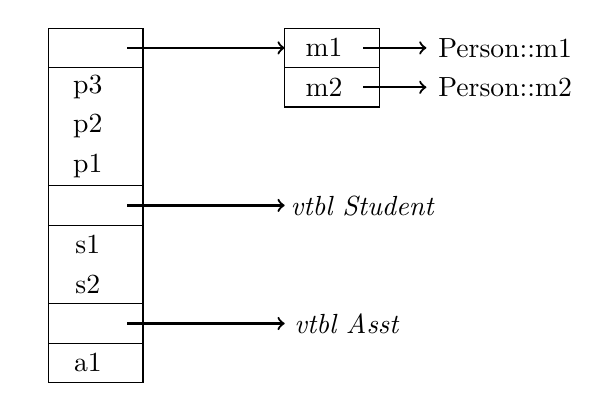
\begin{tikzpicture}

% object 3
\draw (0,-2.5)  rectangle (1.2,-3.0);
\pgftext[at={\pgfpoint{0.5cm}{-2.75cm}}]{a1} ;

% vptr object 3
\draw (0,-2.5)  rectangle (1.2,-2.0);
\pgftext[at={\pgfpoint{0.5cm}{-2.25cm}}]{} ;
\draw[->, thick] (1.0, -2.25) -- (3.0,-2.25); 
\pgftext[at={\pgfpoint{3.8cm}{-2.25cm}}]{\textit{vtbl Asst}} ;

% object 2
\draw (0,-2.0)  rectangle (1.2,-1.0);
\pgftext[at={\pgfpoint{0.5cm}{-1.25cm}}]{s1} ;
\pgftext[at={\pgfpoint{0.5cm}{-1.75cm}}]{s2} ;

% vptr
\draw (0,-1.0)  rectangle (1.2,-0.5);
\pgftext[at={\pgfpoint{-0.25cm}{-0.75cm}}]{} ;
\draw[->, thick] (1.0, -0.75) -- (3.0,-0.75); 
\pgftext[at={\pgfpoint{4.0cm}{-0.75cm}}]{\textit{vtbl Student}} ;

% object 1
\pgftext[at={\pgfpoint{0.5cm}{-0.25cm}}]{p1} ;
\pgftext[at={\pgfpoint{0.5cm}{0.25cm}}]{p2} ;
\pgftext[at={\pgfpoint{0.5cm}{0.75cm}}]{p3} ;
\draw (0,-0.5)  rectangle (1.2,1.5);

% vptr 
\draw (0,1.0)  rectangle (1.2,1.5);
\pgftext[at={\pgfpoint{0.5cm}{1.25cm}}]{} ;
\draw[->, thick] (1.0, 1.25) -- (3.0,1.25); 





% right one 

% vtbl for 

% vtbl for Person
%\draw (3,-0.5)  rectangle (4.2,0.0);
%\pgftext[at={\pgfpoint{3.5cm}{-0.25cm}}]{m4} ;
%\draw[->, thick] (4.0, -0.25) -- (4.8,-0.25); 
%\pgftext[at={\pgfpoint{5.8cm}{-0.25cm}}]{Person::m4} ;


%\draw (3,0)  rectangle (4.2,0.5);
%\pgftext[at={\pgfpoint{3.5cm}{0.25cm}}]{m3} ;
%\draw[->, thick] (4.0, 0.25) -- (4.8,0.25); 
%\pgftext[at={\pgfpoint{5.8cm}{0.25cm}}]{Person:m3} ;

\draw (3,0.5)  rectangle (4.2,1.0);
\pgftext[at={\pgfpoint{3.5cm}{0.75cm}}]{m2} ;
\draw[->, thick] (4.0, 0.75) -- (4.8,0.75); 
\pgftext[at={\pgfpoint{5.8cm}{0.75cm}}]{Person::m2} ;

\draw (3,1.0)  rectangle (4.2,1.5);
\pgftext[at={\pgfpoint{3.5cm}{1.25cm}}]{m1} ;
\draw[->, thick] (4.0, 1.25) -- (4.8,1.25); 
\pgftext[at={\pgfpoint{5.8cm}{1.25cm}}]{Person::m1} ;

\end{tikzpicture}
}
\end{tabular}

\end{tabular}

\end{frame}

\begin{frame}[fragile]
\frametitle{Name clashes (again)}
\framesubtitle{}
If two base classes define a method (field) with the same signature,
the ambiguity must be resolved. 

\begin{itemize}
\item Language-defined priorities
\begin{itemize}
\item CLOS: first-fit
\end{itemize}
\item Prohibited (and checked)
\begin{itemize}
\item Eiffel: error at compile time of the child class
\item Must be resolved manually, e.g., via \texttt{rename}; % or \texttt{select} 
\begin{eiffel}
class COURSE_ASSISTANT
inherit
      STUDENT
          rename
              name as teacher_name
          end
      PERSON
\end{eiffel}
\end{itemize}
\item Ambiguous use prohibited (and checked)
\begin{itemize}
\item \Cpp: no error at class compilation time, but at method invocation
time (statically)
\item Must be resolved manually,  via scope resolution operator
\begin{cplus3}
if (...) person::name() else student::name(); 
\end{cplus3} 
\end{itemize}
\end{itemize}
       select 
          move ..

\end{frame}


\begin{frame}[fragile]
\frametitle{Repeated inheritance}
\framesubtitle{}
In \textit{repeated}  inheritance, a class serves as 
ancestor repeatedly, through multiple inheritance relationships. 

\begin{cplus3}
class A;
class B: public A {...}
class C: public A {.. }
class D: public B, C {...}
\end{cplus3}

Replicated: 
\begin{itemize}
\item  $D$ objects contain 2 copies of $A$ objects
\item \Cpp's default choice. Shared inheritance requires keyword \texttt{virtual}.
\end{itemize}
Shared (``diamond''): 
\begin{itemize}
\item  $D$ objects contain only 1 $A$ object.
\item Eiffel's choice. Replication inheritance only via renaming. 
\end{itemize}

\end{frame}

\begin{frame}[fragile]
\frametitle{Replicated inheritance}
\framesubtitle{}
Default case in \Cpp. 
\begin{cplus3}
class A;
class B: public A {...}
class C: public A {.. }
class D: public B, C {...}
\end{cplus3}


\begin{itemize}
\item Members of $A$ are ambiguous $\leadsto$ no direct access possible
(scope resolution operator doesn't help); access via parents needed.  
\item Virtual function tables are merged  and the portions $C::A$ methods
and $B::A$ methods are kept. 

\mycomment{
\begin{cplus3}
// C++ 
A* b; B* b; C* c; D* d;
a = d; // error
b = d; 
c = d;
a = b;
a = c; 
\end{cplus3}
}
\end{itemize}
\bigskip

Problem: inconsistency
\end{frame}

\begin{frame}[fragile]
\frametitle{Shared inheritance}
\framesubtitle{}
Default case in Eiffel. In \cpp, the keyword \texttt{virtual} 
indicates sharing.
Shared inheritance avoids name clashes between parents.

\begin{cplus3}
class A;
class B: public virtual A {...}
class C: public virtual A {.. }
class D: public B, C {...}
\end{cplus3}



New ambiguity: what if both $B$ and $C$ override a method in $A$?
\begin{itemize}
\item Eiffel: use \texttt{select} to resolve ambiguity
\item \Cpp: compile-time error
\end{itemize}

General problem:


\begin{itemize}
\item In \Cpp, neither child nor virtual parent determine the construction
of parent objects---only grandchildren.
%\item In \Cpp, virtual function table gets either bigger or there is an additional level of indirection.
\item In Eiffel, it depends on the future client whether
a feature will be shared or replicated.
\end{itemize}
$\leadsto$ Implementation quite 
complicated 
\end{frame}

\begin{frame}[fragile]
\frametitle{Mix-in inheritance and interface}
\framesubtitle{}
\textit{Mix-in inheritance} is an alternative to multiple inheritance, but
avoids problems or complications with replicated inheritance.

\begin{itemize}
\item Same motivation: combine \textit{orthogonal} functionality
\item Encapsulate each functionality in a class
\item No superclasses: mix-in classes are in
flat hierarchies 
\item No subclasses:  a mix-in class is for
``mixing in'' properties and cannot be instantiated
\end{itemize}

Example: interfaces in Java and C\#
\end{frame}



\subsection{Binary methods}

\begin{frame}[fragile]
\frametitle{Binary methods}
\framesubtitle{Or in general: n-ary methods}
\begin{itemize}
\item Binary methods take 2 parameters of the same type.
\item 
In OOP, binary methods are methods that contain one or more parameters
of the same type as the receiver object.
\item Examples: arithmetic, equality, comparison, \ldots
\end{itemize}
\bigskip

They cause great difficulties in OOP. 
\end{frame}

\begin{frame}[fragile]
\frametitle{Binary methods problem}
\framesubtitle{Bruce, Cardelli, Hopkins Object Group }
% typing in the presence of inheritance.

Problem: 

\begin{itemize}
\item Receiver and argument are not treated symmetrically (but
should be). 
\end{itemize}


% I do not understand this...
% \bigskip

% Other problems (also big): 

% \begin{itemize}
% \item Retrofitting of new classes not possible (makes extension
% impossible)
% \item Special access rights needed (violates protection)
% %\item Do subclasses always produce subtypes?
% \end{itemize}

\end{frame}

\begin{frame}[fragile]
\frametitle{Asymmetry}
\begin{cplus3}
class Complex 
{
    // add: (Complex , Real) -> Complex  
    public Complex add(Real d) {...}
}
\end{cplus3}
How to define an addition with signature 
\begin{center}
\textit{double × Complex} → \textit{Complex}?
\end{center}
\begin{itemize}
\item Impossible in almost all OO-language (Java, C\#)!
Exception: very few (``multi-dispatch languages'') 
\item Possible in hybrid language (Ada, \Cpp) via non-OO constructs,
e.g., free functions and overloading (or ``friends''). 
\end{itemize}
\end{frame}

\begin{frame}[fragile]
\frametitle{Method dispatching}
\framesubtitle{}

Single-dispatch languages
\begin{itemize}
\item Dispatch based on the (dynamic) class of the receiver. 
\begin{cplus3}
     Complex c = ... ;   
     c.add(arg);
\end{cplus3}
\item Ex.: all languages mentioned so far

\end{itemize}

Multiple-dispatch languages
\begin{itemize}
\item Dispatch (also) based on the dynamic class of \textit{arguments}.
\item Ex.: Dylan (Apple), CLOS, Cecil
\item Deviation from previous class concept: data records + generic functions.
\begin{cplus3}
     add(arg1, arg2);
\end{cplus3}
\item Combined overloading \& overriding (resolution at run time).
\end{itemize} 
\end{frame}

\begin{frame}[fragile]
\frametitle{Multi-methods in Dylan}
\framesubtitle{}
A multi-method is a method that does not belong to one class
\begin{itemize}
\item For each binary method, there exists
a set of method bodies associated with the name of the method.
\item The dispatch depends on all parameter types.
\end{itemize}
\begin{cplus3}
// http://www.opendylan.org/books/dpg/db_88.html
// Generic ``+'' 
// Method on <time-offset>, <time-offset>
define method \+
    (offset1 :: <time-offset>, offset2 :: <time-offset>)
=> (sum :: <time-offset>)
 let sum = offset1.total-seconds + offset2.total-seconds;
 make(<time-offset>, total-seconds: sum);
end method \+;	

// Method on <time-offset>, <time-of-day>
define method \+ 
    (offset :: <time-offset>, time-of-day :: <time-of-day>)
 => (sum :: <time-of-day>)
  make(<time-of-day>, 
       total-seconds: offset.total-seconds + time-of-day.total-seconds);
end method \+;
\end{cplus3}
\end{frame}


\subsection{Overriding in real languages}

\begin{frame}[fragile]
\frametitle{Overriding rules in real languages}
\framesubtitle{}
Overriding can be \textit{covariant}, 
\textit{contravariant}, or \textit{invariant} in either
the argument types or the return type.
\bigskip


Assume a class \texttt{Animal}, a child \texttt{DomesticAnimal} with 
%a method 
%\begin{center} set_playmate(Sandwich) → void \end{center}
\begin{cplus3}
       set_playmate(DomesticAnimal)->  void 
\end{cplus3}

and the child \texttt{Cat},
which re-defines \texttt{set_playmate}. 
How may the argument type change?% (relativeto DomesticAnimal.set_playmate):
\begin{itemize}
\item Covariance (in the argument type):
\begin{cplus3}
 set_playmate(Cat) -> void
\end{cplus3}
 \item Contravariance:
\begin{cplus3}
 set_playmate(Animal) -> void
\end{cplus3}
  \item Invariance: 
\begin{cplus3}
 set_playmate(DomesticAnimal) -> void
\end{cplus3}


\end{itemize}
Eiffel uses the covariance rule; but this can be unsafe (why?).
%http://www.faqs.org/faqs/eiffel-faq/
Most languages use the invariance rule (for argument types). 
\end{frame}

\begin{frame}[fragile]
\frametitle{Covariance in return type}
\framesubtitle{}
Covariance in the return type is less contested.
\bigskip

\begin{cplus3}
// Java 1.5
class BaseClass {
    public BaseClass Clone() {..}
}
class DerivedClass extends BaseClass {
    public DerivedClass Clone() {..}
}
\end{cplus3}
Java, \Cpp, Eiffel support covariance in the return type.\\
C\# requires invariance. 
\end{frame}



\begin{frame}[fragile]
\frametitle{Pre-and postconditions in Eiffel}
\framesubtitle{Restricting replacement semantics}
\textit{Assertion redeclaration rule}: a redeclared version need not contain its own requires or ensure
clause.
\begin{itemize}
\item It may use a \texttt{require else} or
\texttt{then ensure} clause
to weaken/strengthen the pre/postcondition of the parent. 

\end{itemize}
\begin{eiffel}
class ACCOUNT 
feature
   withdraw(sum: INTEGER) is
       require
           sum >= 0
       do ..  end
end -- class ACCOUNT
class SPECIAL_ACCOUNT inherit
      ACCOUNT
      redefine withdraw end
feature
       withdraw(sum: INTEGER) is
       do ...
       ensure then
           balance >= 1000
       end
end -- class SPECIAL_ACCOUNT       
\end{eiffel}
\end{frame}



\end{document}






